\begin{surferIntroPage}{Simple Singularities}{simplesing_A1pm}{Simple Singularities}
This gallery visualizes the most important class of singularities of algebraic surfaces, the so--called Simple or ADE--Singularities.
An (algebraic) surface is the set of points $(x_0, y_0, z_0)$ in real $3$--space (imagine the three--dimensional space in which we live) for which $f(x_0, y_0, z_0)=0$, where $f(x,y,z)$ is a polynomial in the variables $x,y,z$.

Surfaces that look in a small neighbourhood of each point like a plane (they do not have any apex or self--intersection or pieces meeting tangentially) are called non--singular or smooth. Non--smooth points are called singular or singularities.
 Examples of smooth surfaces are a plane, a sphere and a torus (the first 3
    pictures), examples of singular surfaces are $A_1, A_2, A_3$ (the last 3 pictures):
    \begin{center}
      \vspace{-0.25cm}
      \begin{tabular}{@{}c@{}c@{}c@{}c@{\quad}c@{}c@{}c@{}c@{}}
        \begin{tabular}{@{}c@{}}
          smooth:
        \end{tabular}
        &
        \begin{tabular}{@{}c@{}}
          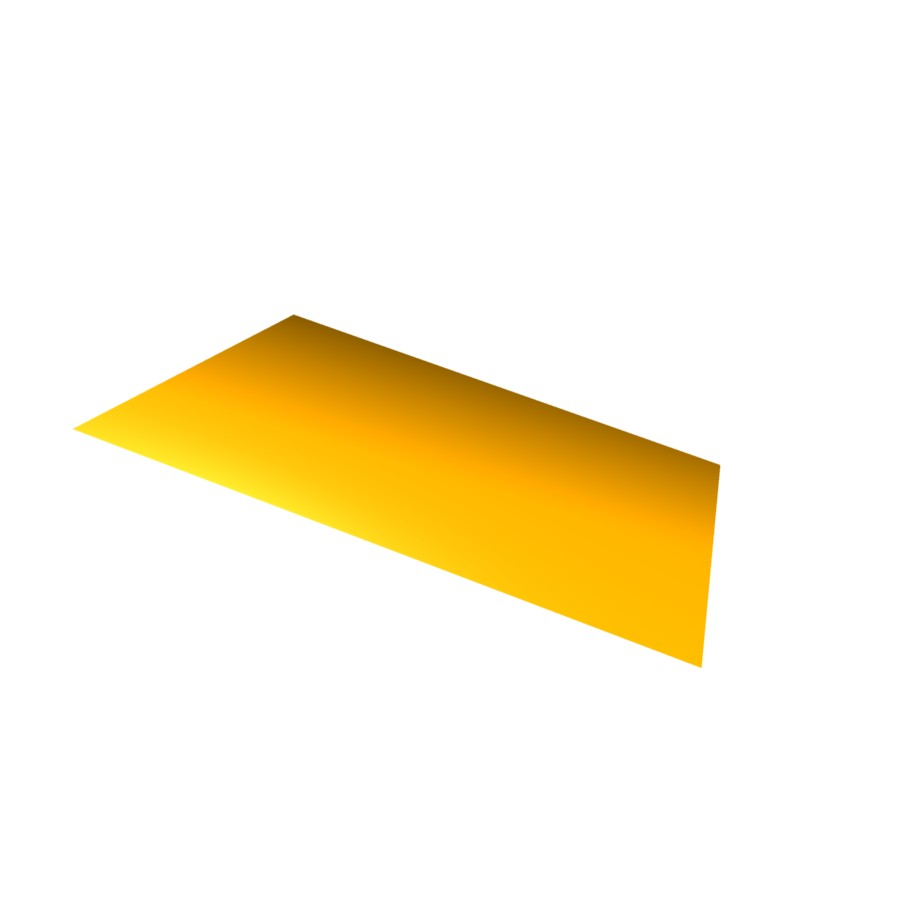
\includegraphics[width=1.1cm]{../../common/images/plane}
        \end{tabular}
        &
        \begin{tabular}{@{}c@{}}
          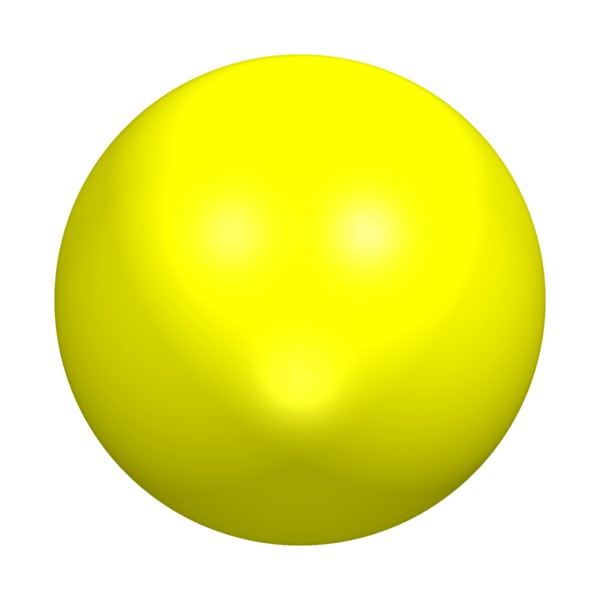
\includegraphics[width=1.1cm]{../../common/images/kugel}
        \end{tabular}
        &
        \begin{tabular}{@{}c@{}}
          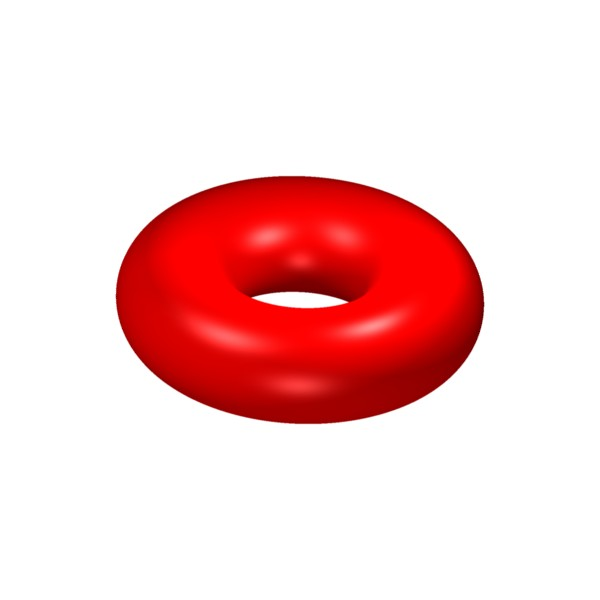
\includegraphics[width=1.1cm]{../../common/images/torus}
        \end{tabular}
        &
        \begin{tabular}{@{}c@{}}
          singular:
        \end{tabular}
        &
        \begin{tabular}{c@{}@{}}
          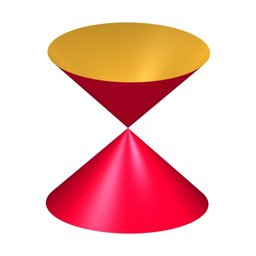
\includegraphics[width=1.1cm]{../../common/images/kegel}
        \end{tabular}
        &
        \begin{tabular}{c@{}@{}}
          \includegraphics[width=1.1cm]{../../common/images/A2pm}
        \end{tabular}
        &
        \begin{tabular}{c@{}@{}}
          \includegraphics[width=1.1cm]{../../common/images/A3pm_0}
        \end{tabular}
      \end{tabular}
    \end{center}
    \vspace{-0.35cm}

The Simple or ADE--Singularities are given by the infinite series $A_k^{\pm\pm}, k\geq 1,$\ $D_k^{\pm\pm}$,  $k\geq 4,$ and the three singularities $E^\pm_6,\ E^\pm_7,\ E^\pm_8.$ These singularities are important since they have amazing relations to numerous different areas of mathematics, to mathematical physics and to real life (e.g. in geometric optics).

Using the Surfer everyone can visualize these singularities. However, the complexity cannot be directly seen from their picture. A better way is to deform the equation slightly (in a special way) and to visualize the deformed surface. Each $A_k$-singularity can be deformed into $\lfloor\frac{k+1}{2}\rfloor$
    $A_1$-singularities; for an $A_3^{+-}$, we obtain two $A_1^{+-}$ (3 pictures on the left):
%    \dontshow{

    \begin{center}
      \vspace{-0.25cm}
      \begin{tabular}{@{}c@{\quad}c@{}c@{\qquad\quad}c@{\quad}c@{\quad}c@{}}
        \begin{tabular}{@{}c@{}}
          \includegraphics[width=1.2cm]{../../common/images/A3pm_0}
        \end{tabular}
        &
        \begin{tabular}{@{}c@{}}
          \includegraphics[width=1.2cm]{../../common/images/A3pm_1}
        \end{tabular}
        &
        \begin{tabular}{@{}c@{}}
          \includegraphics[width=1.2cm]{../../common/images/A3pm_2}
        \end{tabular}
        &
        \begin{tabular}{@{}c@{}}
          \includegraphics[width=1.2cm]{../../common/images/A3pm_vz_2}
       \end{tabular}
        &
        \begin{tabular}{@{}c@{}}
          \includegraphics[width=1.2cm]{../../common/images/A3pm_vz_1}
        \end{tabular}
        &
        \begin{tabular}{@{}c@{}}
          \includegraphics[width=1.2cm]{../../common/images/A3pm_vz_0}
        \end{tabular}
      \end{tabular}
      %\begin{tabular}{@{}c@{\qquad\qquad}c@{}}
      %    $A_3 \qquad\quad \rightarrow \qquad 2 A_1$
      %    &
      %    $2$ Zykel $+$ $1$ Zykel \ $\rightarrow \ A_3$
      %  \end{tabular}
    \end{center}
%   }
    \vspace{-0.4cm}
    The index $k$ of the $A_k$--singularities is the so--called \emph{Milnor
      Number} of the singularity; this is the number of \emph{holes} which vanish when contracting them to the singular point (pictures on the right).

%For a deeper understanding of these singularities one needs actually complex nu%mbers, i.e. the points $(x_0, y_0, z_0)$ of the ''surface'' $f(x,y,z)=0$ lie in% complex $3$--spaces (real $6$--space), bus this cannot be visualized.
\end{surferIntroPage}
